\section{Contributions}
We provide a prediction-based solution to support efficient and consistent concurrency control. Our approach is based on building a reputation for each transaction using its efficiency rate (i.e., computational cost) and the outcome (i.e., commit or abort). Using these properties transactions are categorized into four categories. The priorities associated with each category impact the transaction's scheduling. Our aim is to prevent cascading rollbacks and inconsistent database state while supporting practical concurrency control. We provide new lock types corresponding to transaction categories. Using these locks transaction scheduler will be able to determine which lock requests to permit. These eventually determine transaction scheduling, delays, and aborts. Our expectation is that prediction-based scheduling will increase both efficiency and consistency.

We identified two research areas in the context of prediction-based scheduling within web service environments that need to be addressed. These are:
\begin{itemize}
    \item transactional correctness within concurrency control
    % \item predictions within multi-level secure databases
    \item dynamic reputation for transactions
    % \item prediction-based scheduler within linked databases
\end{itemize}

\subsection{Transactional Correctness}
In this work we developed the theoretical foundation for the prediction-based scheduling. This included the development of a framework, associated concepts, and technologies. A completely new concurrency control paradigm was developed in order to elevate particular transactions over others. In this paradigm there are three actions used to determine the course of action for a particular transaction. These three actions either grant, elevate, or decline an transaction to enable concurrent operations and prevent deadlock. By ensuring the transactional correctness within the prediction-based solution, we can then use this foundation to build upon in regards to other research areas. The work discussed in this area is documented in Chapter \ref{chap:prediction_based_scheduler}.

\begin{figure}[h]
\captionsetup{justification=centering}
\centering
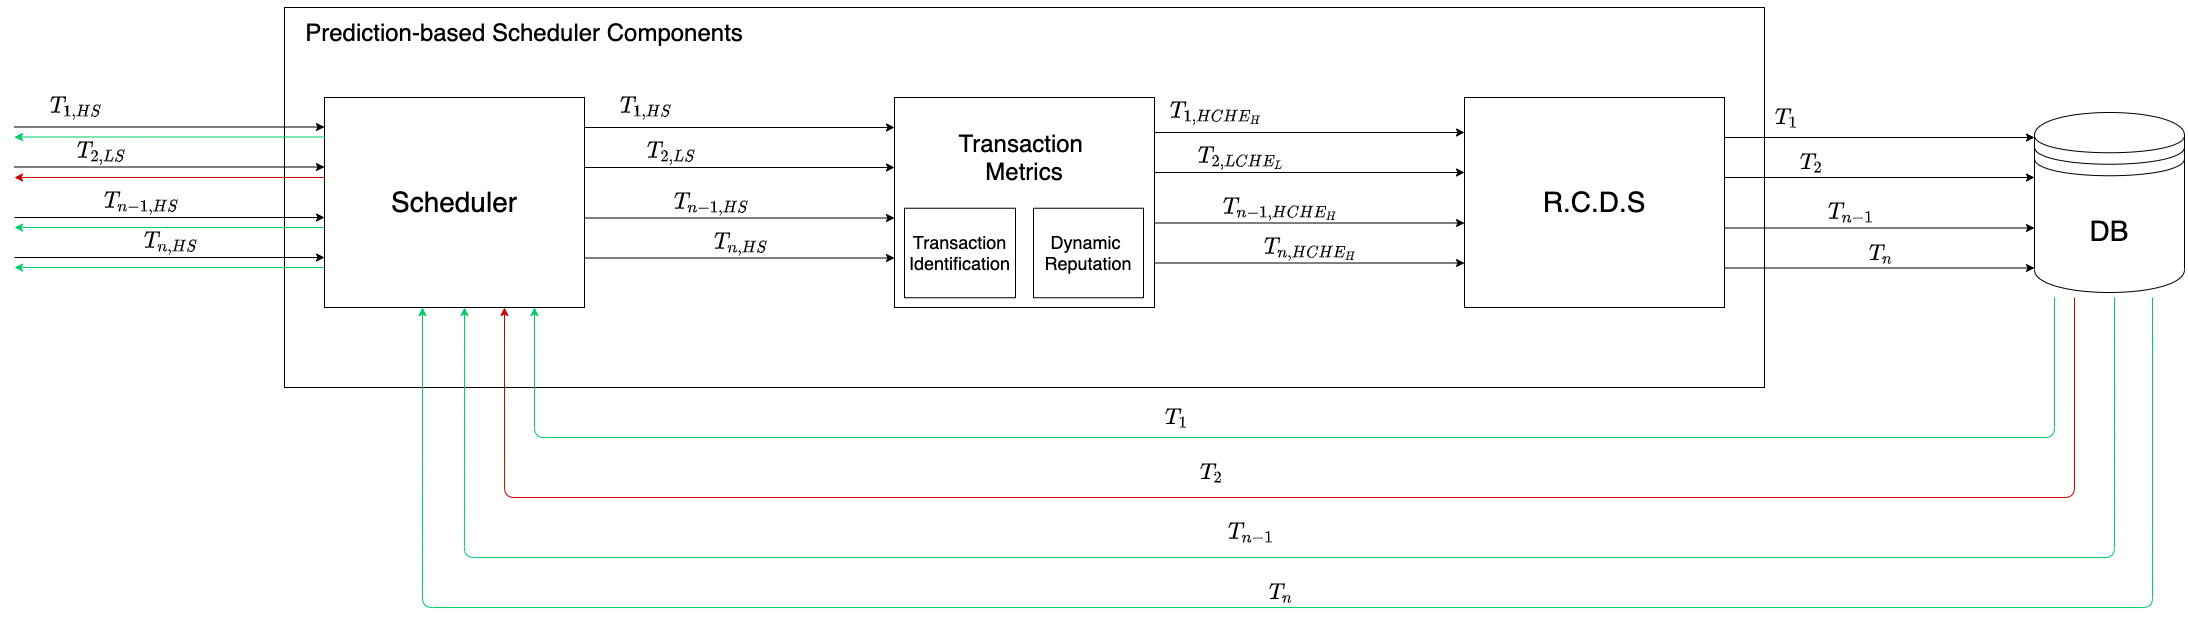
\includegraphics[width=\textwidth]{images/SystemModel_Overall}
\caption{Overall System Model of Prediction-based Scheduler}
\label{fig:system_model_overall}
\end{figure}

\subsection{Dynamic Reputation for Transactions}
In the previous section, the categorization of the transaction is assumed in order to continue forward with the decision model. This section of the dissertation involves the work needed to establish a dynamic reputation management system to allow for dynamic reputation. It involves building a reputation score for each transaction based on the transactions ranking of efficiency, commits, system aborts, and user aborts. Once a reputation score is provided we can then use dynamic reputation management to dynamically promote and demote transactions. This then allows the system to adapt to its environment dynamically. The work discussed in this area is documented in Chapter \ref{chap:dynamic_reputation}.

% Figure \ref{fig:system_model_overall} displays the system model for the work done for transactional correctness and building a dynamic reputation for transactions.